\chapter{Generating Fractals using Geometric Algebra}

Fractals have always been a popular topic in computer graphics due to their
ability to give rise to great aesthetic beauty from a relatively simple
mathematical description. Generally a fractal is considered to be any
geometric object which posesses detail on all
scales\cite{FRAC:FractalsEverywhere, FRAC:FractalGeometryOfNature}. That is to
say that one may examine the edge of the object under arbitrary magnification
yet still find it rough and irregular. Many introductions to the subject of
fractals and their creation on computers exist\cite{FRAC:FractalGeometry,
  FRAC:ChaosAndFractals, FRAC:FractalImages}.

The term fractal was coined by Mandelbrot\cite{FRAC:LesObjetsFractals} in 1975,
originally from the latin {\em fractus} (broken). In this chapter we
investigate an extension into GA of the class of fractals he is most 
associated with which are based on repeated iteration of a complex function.
Fractals have found applications in a wide selection of research areas
including image compression (FIXME Citation) and it is supected that the 
GA-based approach here may also be of use in a similar manner.

\section{Fractals from Complex Iteration}

\begin{figure}
\centering
\begin{tabular}{c@{$\quad$}c}
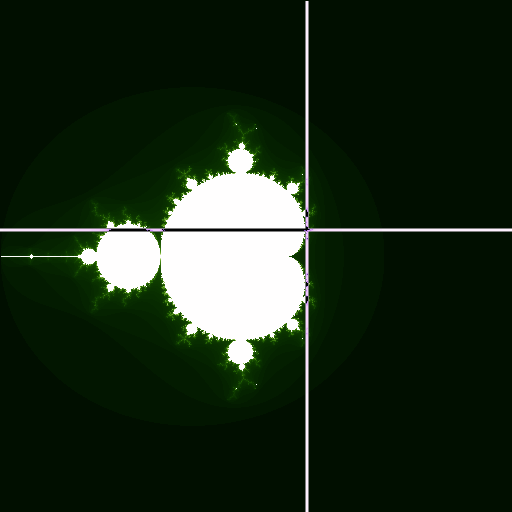
\includegraphics[width=0.4\textwidth]{euc_mandel_julia_pos} 
 & 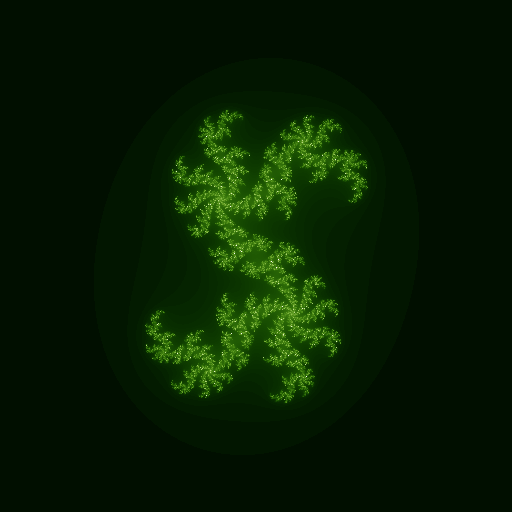
\includegraphics[width=0.4\textwidth]{julia_euc} \\
                          (a) & (b)
\end{tabular}
\caption{\label{fig:euclidean_sets}The well known (a) Mandelbrot set with
  the constant $c = 0.4 + 0.2i$ marked and (b) the Julia
  set associated with $c$.}
\end{figure}

The Mandelbrot and Julia sets (figure \ref{fig:euclidean_sets}) are well known, even to
laymen, as examples of fractals. They are, in actual fact, examples of a 
common form of fractals known `recurrence' or `escape-time' fractals.
Such fractals are generated by iterating some complex function and noting
how fast it `escapes' to infinity (if at all).
The Mandelbrot and Julia sets are both generated using the following 
complex recurrence relation\cite{FRAC:Mandelbrot, FRAC:JuliaMandelBook}:
\begin{definition}
The complex function $z(n,c)$, $n \in {\mathbb Z}^+, c \in {\mathbb C}$,
    is defined as
\[
z(n,c) = z^2(n-1,c) + c.
\]
\end{definition}

\subsection{The Mandelbrot Set}

Both the Mandelbrot and Julia sets are generated in a similar manner.

\begin{definition}[The Mandelbrot set]
The Mandelbrot set, $\mathbb{M}$, is defined as
\[
\mathbb{M} = 
\left\{x \in \mathbb{C} 
: \lim_{n \rightarrow \infty} \magof{z(n,x)} < \infty \right\} 
\]
where $\magof{\cdot}$ is the usual Euclidean $2$-norm and $z(0,c) = 0$.
\end{definition}

After a little work one may readily convince onself that if $\magof{z(n,x)} \ge 2$
for some $n$ and $x$ then $\magof{z(n,x)} \rightarrow \infty$ as $n \rightarrow \infty$.
Hence we may determine if some point $x$ is \emph{not} as soon as if $\magof{z(n,x)} \ge 2$. 
In practice one may have to wait an arbitrarily long time for this condition to be met
and one will never obtain it if $x$ is within the set. We generally approximate the
set by choosing some maximum number of iterations to wait before labelling
$x$ as being within the set. We shall assume that we can identify a complex number $c$ 
with any point in the image plane, usually by setting $c = x + yi$ for pixel
$(x,y)$ and scaling the co-ordinate system such that the region of interest of
the complex plane is within the image.  Our algorithm for generating an image of the
set is shown in algorithm \ref{alg:generate_mandelbrot}.

\begin{fancyalg}
\begin{algorithmic}[1]
\STATE $i_{\mbox{max}} :=$ maximum number of iterations
\FORALL{$c \in {\mathbb C}$ in image}
\STATE $z := c$
\STATE $i := 0$
\WHILE{$zz^* < 4$ and $i < i_{\mbox{max}}$}
  \STATE $z := z^2 + c$
  \STATE $i := i+1$
\ENDWHILE 
\STATE set pixel $c$ to colour $i$
\ENDFOR
\end{algorithmic}
\caption{
\label{alg:generate_mandelbrot}
  Generating the Mandelbrot set}
\end{fancyalg}

The level of detail of the resulting image being determined by the value of $i_{\mbox{max}}$.
The image of the Mandelbrot set in figure \ref{fig:euclidean_sets}a was
generated with $c = x + yi$ and $x \in (-2,2), y \in (-2,2)$.

In figure \ref{fig:euclidean_sets}a a colour palette was chosen so that colour 0 was black
and colour $i_{\mbox{max}}$ was white moving through dark-green. The brightness of
each pixel is therefore some measure of how long it took to decide whether that point was
a member of the set.

\subsection{The Julia Set}

There are an infinite number of Julia sets, each associated with
a particular point on the complex plane. The definition of the Julia set is somewhat
similar to that of the Mandelbrot set.

\begin{definition}[The Julia set]
The Julia set associated
with the complex number $c$, $\mathbb{J}_c$, is given by
\[
\mathbb{J}_c = 
\left\{x \in \mathbb{C}
: \lim_{n \rightarrow \infty} \magof{z(n,c)} < \infty \right\} 
\]
where $z(0,c) = x$.
\end{definition}

The difference between this and the Mandelbrot set is that there exists a 
Julia set associated with each complex number. This constant must be chosen before
generating the image. Our algorithm for generating Julia sets is, as one would
expect, similar to that for the Mandelbrot set and is shown in algorithm
\ref{alg:generate_julia}.

\begin{fancyalg}
\begin{algorithmic}[1]
\REQUIRE{$c =$ constant}
\STATE $i_{\mbox{max}} :=$ maximum number of iterations
\FORALL{$z \in {\mathbb C}$ in image}
\STATE $i := 0$
\WHILE{$zz^* < 4$ and $i < i_{\mbox{max}}$}
  \STATE $z := z^2 + c$
  \STATE $i := i+1$
\ENDWHILE 
\STATE set pixel $z$ to colour $i$
\ENDFOR
\end{algorithmic}
\caption{
\label{alg:generate_julia}
  Generating the Julia set}
\end{fancyalg}

Due to their similarity there exist a number of theorems and conjectures which link the
Mandelbrot and Julia sets in some way. For example, if $c \in \mathbb{M}$ then
the Julia set $\mathbb{J}_c$ is connected(FIXME Citation). If $c$ is near the 
border of $\mathbb{M}$ then it is a Cantor set(FIXME Citation).

\section{Extending Complex Numbers}

In this section we will seek to find a co-ordinate free analogue to the
complex mapping $z \mapsto z^2$ in order to re-cast the fractals above in
terms of geometric operations using GA. We will start by confining ourselves
to the complex plane and then move into higher dimensions.

We start by defining a mapping between the complex numbers, $\mathbb{C}$, and
the vector-space of the complex plane, $\mathbb{R}^2$. Letting $\{e_1, e_2\}$
be some orthonormal basis for $\mathbb{R}^2$ we can form a natural one-to-one
mapping between $z \in \mathbb{R}^2$ and $C(z) \in \mathbb{C}$:

\begin{definition}
Given some vector $z \in \mathbb{R}^2$, we can map one-to-one into the
complex plane by forming the complex number
\[
C(z) = (z \cdot e_1) + (z \cdot e_2)i.
\]
\end{definition}

Here it is clear that $e_1$ corresponds to the real-axis and $e_2$ 
corresponds to the imaginary axis of the complex plane.
It is now trivial to show that
\begin{align*}
C^2(z) &= [(z \cdot e_1) + (z \cdot e_2)i]^2 \\
       &= (z \cdot e_1)^2 - (z \cdot e_2)^2 + 2(z \cdot e_1)(z \cdot e_2)i
\end{align*}
which is analgous to the usual method of squaring complex numbers.

\begin{lemma}
Given some vector $z \in \mathbb{R}^2$ representing the complex number
$C(z)$, the mapping $z \mapsto ze_1$ is equivalent to $C(z) \mapsto C^2(z)$.
\end{lemma}
\begin{proof}
Let $z = xe_1 + ye_2$. Therefore $C(z) = x + yi$. It is clear that
\begin{align*}
ze_1z &= (x^2 - y^2) e_1 + 2xye_2 \\
\Rightarrow\;C(ze_1z) &= (x^2 - y^2) + 2xyi\\
        &= C^2(z)
\end{align*}
as required.
\end{proof}

To complete the extension one must also define a geometric equivalent of
addition:
\begin{lemma}
Given vectors $z, c \in \mathbb{R}^2$ representing the complex numbers
$C(z)$ and $C(c)$, the mapping $z \mapsto z + c$ is equivalent to 
$C(z) \mapsto C(z) + C(z)$.
\end{lemma}
\begin{proof}
Clear by direct substitution.
\end{proof}

\section{Moving to Higher Dimensions}

We extend this analogy to cover vectors in $\mathbb{R}^n$ 
by simply removing the constraint that the vectors need be in $\mathbb{R}^2$.

\begin{definition}
Given a vector $z$ and some unit basis vector $e_1$ the mapping
$z \mapsto ze_1z$ is the geometric analogue of squaring a complex number.
\end{definition}

\begin{definition}
Given two vectors, $z$ and $c$, the geometric analogue of complex addition
is $z \mapsto z + c$.
\end{definition}

We may now define generalised Mandelbrot and Julia sets based upon
a new vector recurrence relation.

\begin{definition}
The vector analogue of $z(n,c)$ is defined as
\[
z_v(n,c) = z_v(n-1,c) e_1 z(n-1,c) + c
\]
with initial values being defined by a particular fractal.
\end{definition}

\subsection{The Generalised Mandelbrot Set}

\begin{figure}
\centering
\begin{tabular}{c@{$\quad$}c}
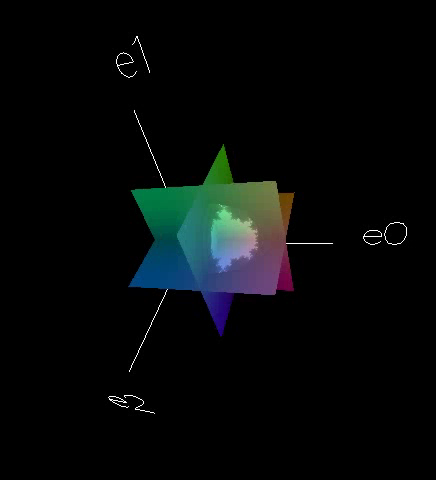
\includegraphics[width=0.4\textwidth]{3dmandel1}
 & 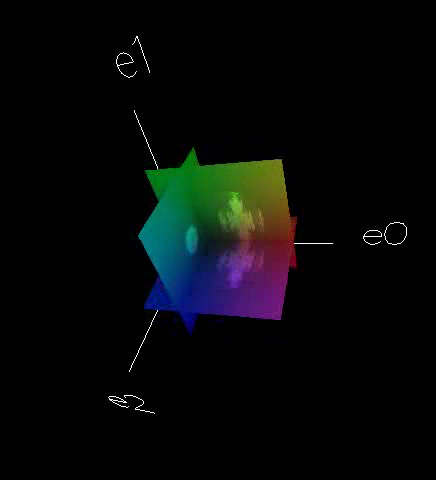
\includegraphics[width=0.4\textwidth]{3dmandel2} 
\end{tabular}
\caption{\label{fig:3dmandel}
  Two frames from an animation\cite{FRAC:MandelAnim} showing slices through
          the 3 dimensional Mandelbrot set.}
\end{figure}

\begin{definition}[The generalised Mandelbrot set]
The generalised Mandelbrot set, $\mathbb{M}_k$, in $\mathbb{R}^k$ 
    is defined as
\[
\mathbb{M}_k = 
\left\{x \in \mathbb{R}^k 
: \lim_{n \rightarrow \infty} z_v^2(n,x) < \infty \right\} 
\]
where $z(0,c) = 0$.
\end{definition}

\subsection{The Generalised Julia Set}

\begin{figure}
\centering
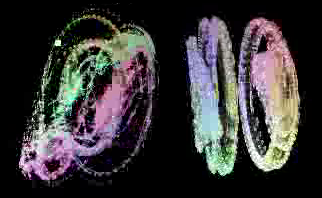
\includegraphics[width=0.4\textwidth]{3djulia_pair.png}
\caption{\label{fig:3djulia}
  Two frames from an animation\cite{FRAC:JuliaAnimation} showing voxel
          rendering of 3d Julia sets.}
\end{figure}

\begin{definition}[The generalised Julia set]
The generalised Julia set, $\mathbb{J}_{c,k}$, in $\mathbb{R}^k$
which is associated with the vector $c \in \mathbb{R}^k$ is given by
\[
\mathbb{J}_{c,k} = 
\left\{x \in \mathbb{R}^k
: \lim_{n \rightarrow \infty} z_v^2(n,c) < \infty \right\} 
\]
where $z(0,c) = x$.
\end{definition}

\subsection{Ray Tracing}

\section{Moving to Hyperbolic Geometry}

\begin{figure}
\centering
\begin{tabular}{c@{$\quad$}c}
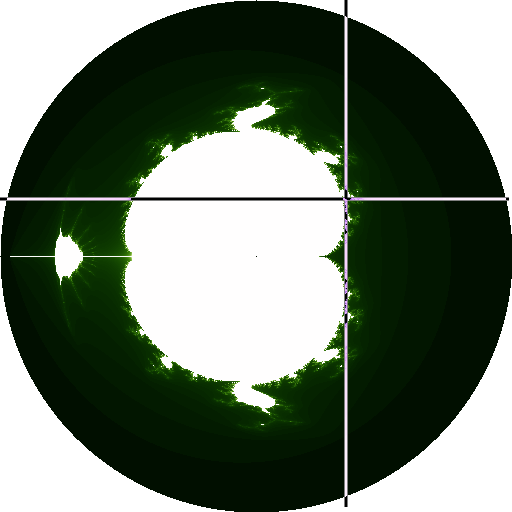
\includegraphics[width=0.4\textwidth]{hyp_mandel_julia_pos} 
 & 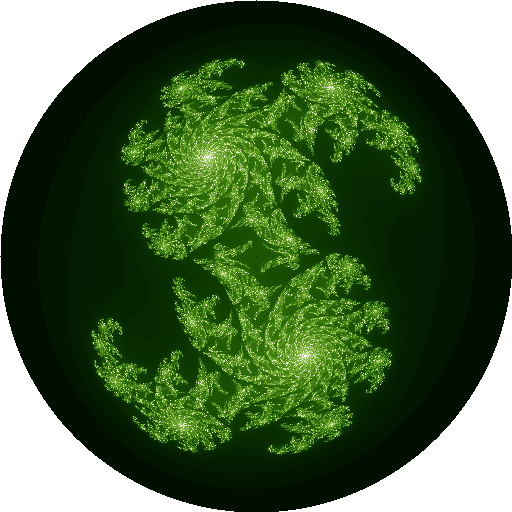
\includegraphics[width=0.4\textwidth]{julia_hyp} \\
                          (a) & (b)
\end{tabular}
\caption{\label{fig:noneuclidean_sets}The non-Euclidean analogue of the (a) Mandelbrot set with
  the constant $c = 0.4e_1 + 0.2e_2$ marked and (b) the Julia
  set associated with $c$.}
\end{figure}

\subsection{The Hyperbolic Mandelbrot Set}

\subsection{The Hyperbolic Julia Set}
